\documentclass[tikz,convert={outfile=\jobname.svg},border=3mm]{standalone}
%% http://tex.stackexchange.com/questions/197887/how-to-draw-a-system-architecture-with-databases-and-shadows

%% \documentclass[crop,tikz,convert={outext=.svg,command=\unexpanded{pdf2svg \infile\space\outfile}},multi=false]{standalone}

%% \documentclass[tikz,convert={outfile=\jobname.svg}]{standalone}

%% \documentclass[dvisvgm]{standalone}
%% \documentclass[]{minimal}
%% \documentclass[tikz,convert={outfile=\hequality\.svg}]{standalone}


\usepackage{tikz}
\usetikzlibrary{backgrounds,calc,shadows,positioning,fit,matrix,shapes.geometric, shapes.arrows} % add shadows #1

% a way to cut shadows in a cell #2
%http://tex.stackexchange.com/questions/129318/remove-drop-shadow-from-one-node
\makeatletter
\tikzset{no shadows/.code=\let\tikz@preactions\pgfutil@empty}
\makeatother

\tikzset{background/.style={rectangle, inner sep=0.1cm},
  backgroundN/.style={rectangle, fill=white, inner sep=0.3cm},
  backgroundNN/.style={rectangle, fill=red!10, inner sep=0.2cm}}

\definecolor{mybluei}{RGB}{124,156,205}
\definecolor{bluedk}{RGB}{73,121,193}
\definecolor{mygreen}{RGB}{202,217,126}
\definecolor{mypink}{RGB}{233,198,235}

\newcommand\widernode[5][widebox]{
  \node[
    #1,
    fit={(#2) (#3)},
    label=center:{\sffamily\bfseries\color{black}#4}] (#5) {};
}

\begin{document}

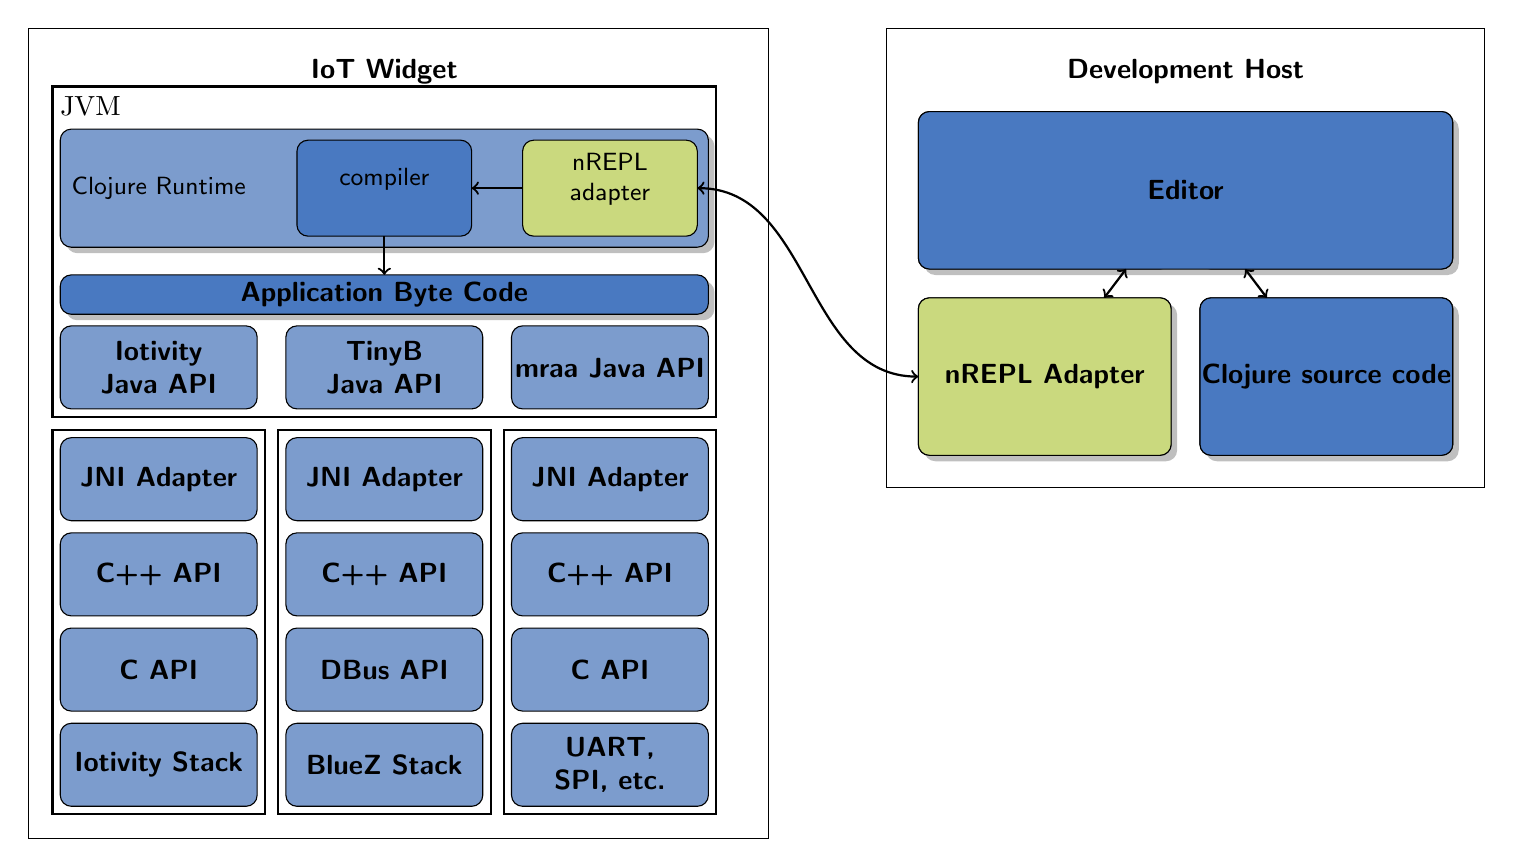
\begin{tikzpicture}[node distance=2pt,outer sep=0pt, % just do nothing after modification
    boxstyle/.style={
      draw=black,
      fill=#1,
      rounded corners,  % drop shadow, %to get a shadow in below a node
      font={\sffamily\bfseries\color{black}},
      align=center,
      minimum height=30pt
    },
    box/.style={
      boxstyle=#1,
      text width=2.5cm},
    box/.default=mybluei,
    title/.style={font={\sffamily\bfseries\color{black}}},
    widebox/.style={draw=black,inner sep=0pt, rounded corners,fill=#1,drop shadow,align=center},
    widebox/.default=mybluei,
    mylabel/.style={font={\sffamily\bfseries\color{black}}},
    database/.style={
      cylinder,
      cylinder uses custom fill,
      cylinder body fill=yellow!50,
      cylinder end fill=yellow!50,
      shape border rotate=90,
      aspect=0.25,
      draw
    }
  ]

  \matrix (widget) [draw=black,%  boxstyle=mybluei!40,%will overpaint blocks with background
    column sep=10pt, row sep=4pt, inner sep=4mm,%
    matrix of nodes,
    anchor=north,
    nodes={box, outer sep=0pt, anchor=center, inner sep=0pt},%
    nodes in empty cells=false,% #3
    row 1/.style={nodes={fill=none,draw=none,minimum height=3mm}},
    row 2/.style={nodes={fill=none,align=left,draw=none,minimum height=3mm}},
    row 3/.style={nodes={fill=none,align=left,draw=none,minimum height=15mm}},
    row 4/.style={nodes={fill=none,align=center,draw=none,minimum height=5mm}}
  ] {
    |[no shadows]| & |[no shadows]| & |[no shadows]| & \\
    |[font={\normalfont\color{black}}] {JVM};| & || & || \\
    |[no shadows]| & |[no shadows]| & |[no shadows]| & \\[6pt]
    || & || & || & \\
    Iotivity Java API & TinyB Java API & mraa Java API & \\[6pt]
    JNI Adapter & JNI Adapter & JNI Adapter & \\
    C++ API & C++ API & C++ API & \\
    C API & DBus API & C API  & \\
    Iotivity Stack & BlueZ Stack & UART, SPI, etc. & \\
  };

  \widernode[]{widget-1-1}{widget-1-3}                  {IoT Widget}{iot-full} %#5
  \widernode[widebox=mybluei]{widget-3-1}{widget-3-3} {}{cljrt} %#5
  \widernode[widebox=bluedk]{widget-4-1}{widget-4-3}    {Application Byte Code}{abc}

  %% \widernode[widebox=green]{widget-3-1}{widget-3-1} {compiler}{cljrt} %#5
  %% \widernode[widebox=green]{widget-3-3}{widget-3-3} {nREPL protocol adapter}{cljrt} %#5

  \draw (widget-3-1) node [font={\sffamily\small\color{black}}] {Clojure Runtime};

  \node[draw,
    text width=minimum width,
    align=center,
    anchor=south,
    distance=2pt,
    inner sep=-4pt,
    rounded corners,
    fill=bluedk,
    font={\sffamily\small\color{black}},
    fit={(widget-3-2)(widget-3-2)}] (compiler) {compiler};

  \node[draw,
    %% text height=4mm,
    %% text depth=2mm,
    text width=minimum width,
    align=center,
    %% minimum height=6mm,
    %% minimum size=6mm,
    anchor=south,
    distance=2pt,
    inner sep=-4pt,
    %% outer sep=-4mm,
    rounded corners,
    %% xshift=5mm,
    fill=mygreen,
    font={\sffamily\small\color{black}},
    fit={(widget-3-3)(widget-3-3)}] (nrepl) {nREPL\\ adapter};


  \draw[->,thick] (nrepl) -- (compiler);
  \draw[->,thick] (compiler) -- (widget-4-2);

  %% \draw (widget-2-1) {JVM};
  %% \widernode[xshift=3em,text width=3em,widebox=mygreen]{widget-2-3}{widget-3-3}   {nrepl}{app}
  %% \node[xshift=3em,inner sep=0pt,text width=3em,draw] {nrepl};
  %% \widernode[widebox=bluedk]{widget-3-1}{widget-3-3}   {Iotivity C++ Layer}{iot-cxx}
  %% \widernode[widebox=bluedk]{widget-5-1}{widget-5-1}      {CoAP}{coap}
  %% \widernode[widebox=bluedk]{widget-6-1}{widget-6-1}      {UDP/IP}{udpip1}

  %%%% blocks

  % jvm
  \begin{pgfonlayer}{background}
    \coordinate (jvm) at (widget-2-1.east);
    %% \coordinate (oth) at (widget-4-3.east);
    \node [thick,background,fit=(widget-2-1) (widget-5-3) (jvm), draw] {};
    %% \node [background,fit=(widget-5-3) (widget-6-3) (oth), draw] {};
  \end{pgfonlayer}

  % tinyb
  \begin{pgfonlayer}{background}
    \coordinate (iot) at (widget-6-1.east);
    \coordinate (tinyb) at (widget-6-2.east);
    \coordinate (mraa) at (widget-6-3.east);
    \node [thick,background,fit=(widget-6-1) (widget-9-1) (iot), draw] {};
    \node [thick,background,fit=(widget-6-2) (widget-9-2) (tinyb), draw] {};
    \node [thick,background,fit=(widget-6-3) (widget-9-3) (mraa), draw] {};
  \end{pgfonlayer}


  \begin{scope}[xshift=10cm]
  \matrix (thinstack) [draw=black,%  boxstyle=mybluei!40,%will overpaint blocks with background
    column sep=10pt, row sep=10pt, inner sep=4mm,%
    matrix of nodes,
    anchor=north,
    nodes={box, align=center, text=black, fill=bluedk, text width=3cm,
      minimum height=2cm,
      outer sep=0pt, anchor=center, inner sep=3pt},%
    nodes in empty cells=false,% #3
    row 1/.style={nodes={fill=none,draw=none,minimum height=3mm}}
    %% yshift=-.75cm,
    %% right=1cm of widget
  ] {
    || & || \\
    || & || \\  % [fill=mygreen]| Editor \\
    || & || \\
  };
  \widernode[]{thinstack-1-1}{thinstack-1-2} {Development Host}{devhost}
  \widernode[widebox=bluedk]{thinstack-2-1}{thinstack-2-2} {Editor}{editor}
  \widernode[widebox=mygreen]{thinstack-3-1}{thinstack-3-1} {nREPL Adapter}{ednrepl}
  \widernode[widebox=bluedk]{thinstack-3-2}{thinstack-3-2} {Clojure source code}{clj-src}
  \end{scope}

  %% \coordinate (foo) at ($(udpip2) + (0,-2)$);
  %% \coordinate (midpt) at ($ (udpip1)!.5!(udpip2) + (0,-1.5) $);

  %% ed
  \draw[<->,thick] (editor) -- (ednrepl);
  \draw[<->,thick] (editor) -- (clj-src);

  %% nrepl comm
  \draw[<->,thick] (ednrepl) to[out=180,in=0] (nrepl);

\end{tikzpicture}

\end{document}
